\lstdefinelanguage{plaintext}{
  sensitive=false,
  comment=[l]{//},
  morecomment=[s]{/*}{*/},
  identifierstyle=\color{black},
  morestring=[b]',
  morestring=[b]"
}

\lstset
{ 
    language=plaintext,
    basicstyle=\footnotesize,
    numbers=left,
    stepnumber=1,
    showstringspaces=false,
    tabsize=1,
    breaklines=true,
    breakatwhitespace=false,
    frame=leftline
}



\chapter{Perancangan}
\label{chap:Perancangan}

Pada bab ini dijelaskan mengenai perancangan perangkat lunak yang dibangun, meliputi perancangan kelas dan perancangan antarmuka.

\section{Perancangan Kelas}
\label{sec:perancangan_kelas}
\begin{figure}[H]
	\centering
		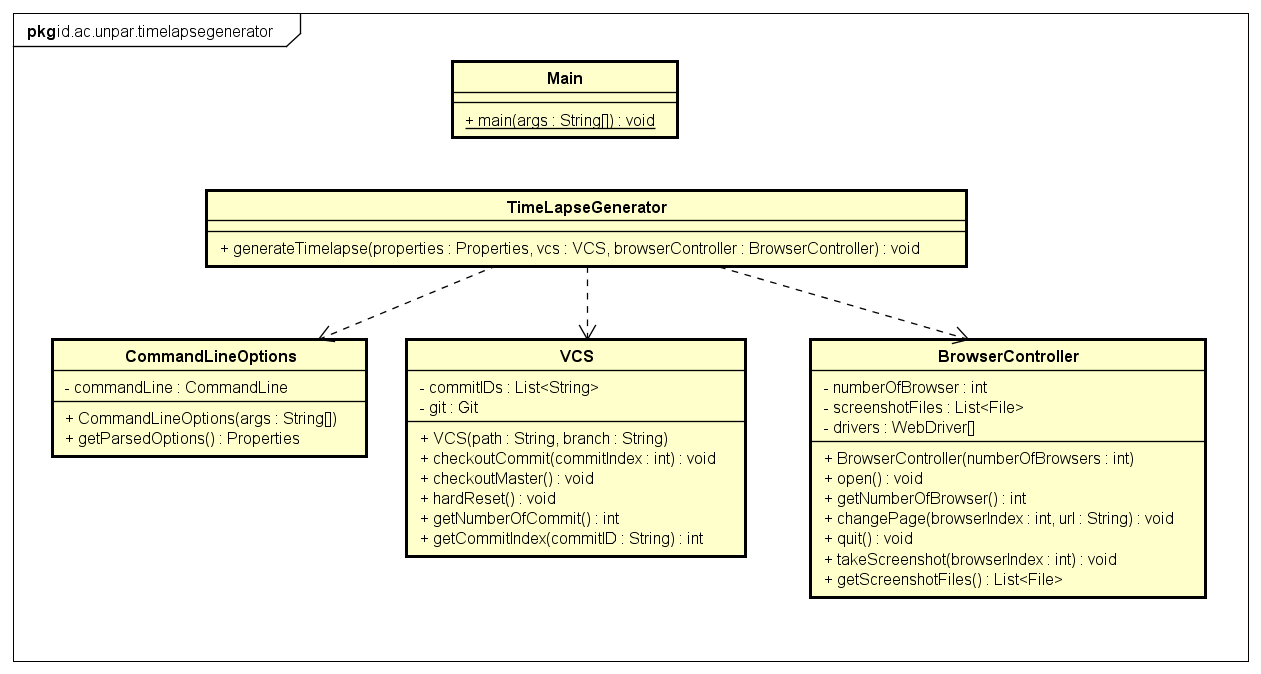
\includegraphics[scale=0.5]{Gambar/ClassDiagram.png}
	\caption{Diagram kelas.}
	\label{fig:class_diagram}
\end{figure}

Program pada skripsi ini memiliki lima kelas. Diagram kelas pada program ini dapat dilihat pada Gambar \ref{fig:class_diagram}. Berikut adalah rincian kelas yang terdapat pada program ini:
\begin{itemize}
\item BrowserController\\
Kelas ini digunakan untuk mengatur \textit{browser}. Operasi-operasi yang dilakukan terhadap \textit{browser} yaitu membuka \textit{browser}, mengambil \textit{screenshot}, membuat \textit{browser window} menjadi maksimal, dan menutup \textit{browser}. Berikut adalah atribut yang terdapat pada kelas ini:
\begin{itemize}
   \item private final WebDriver[] drivers\\
   Atribut ini adalah kumpulan \textit{browser} yang digunakan untuk keperluan \textit{automation testing}. 
    \item private final List<File> screenshotFiles\\
	Atribut ini berfungsi untuk menyimpan \textit{file} hasil \textit{screenshot}.
	\item  private final int numberOfBrowser\\
	Atribut ini menyatakan jumlah \textit{browser} yang dimiliki oleh kelas ini. Jumlah maksimal dari \textit{browser} adalah empat.
\end{itemize}

Berikut adalah \textit{method} yang terdapat pada kelas ini:
\begin{itemize}
\item public BrowserController(int numberOfBrowsers)\\
Constructor dari kelas ini. Berfungsi untuk menginisialisasi atribut yang dimiliki oleh kelas ini. Parameternya adalah jumlah \textit{browser} yang dapat dimiliki oleh kelas ini.
  \item public void open()\\
  Berfungsi untuk membuka semua \textit{browser}, kemudian mengatur ukuran \textit{browser window} menjadi maksimal. 
  \item public int getNumberOfBrowser()\\
  Berfungsi untuk mengembalikan jumlah browser yang dimiliki kelas ini.
  \item public void changePage(int browserIndex, String url)\\
  Berfungsi untuk berpindah halaman pada \textit{browser} tertentu. Parameternya adalah alamat URL untuk berpindah halaman dan indeks \textit{browser} yang akan diubah halamannya.
  \item public void quit()\\
  Berfungsi untuk menutup semua \textit{browser}.
  \item public void takeScreenshot(int browserIndex)\\
  Berfungsi untuk mengambil \textit{screenshot} pada \textit{browser} tertentu dan menyimpannya ke atribut screenshotFiles. Parameternya adalah indeks \textit{browser} yang akan diambil screenshotnya.
\end{itemize}

\item CommandLineOptions\\
Kelas ini berfungsi untuk menyimpan semua Option yang terdapat dalam program ini, dan melakukan \textit{parsing} argumen Command Line Options yang dimasukkan oleh \textit{user}.  

Berikut adalah atribut yang terdapat pada kelas ini:
\begin{itemize}
    \item private final CommandLine commandLine\\
    Atribut ini berfungsi untuk melakukan \textit{parsing} argumen Command Line Options dan menampung hasilnya. 
\end{itemize}
Berikut adalah \textit{method} yang terdapat pada kelas ini:
\begin{itemize}
\item public CommandLineOptions(String[] args)\\
Merupakan Constructor dari kelas ini. Berfungsi untuk menentukan Option yang terdapat pada program dan melakukan parsing argumen Command Line. Parameternya adalah argumen Command Line Option yang didapatkan dari
kelas Main.
\item public Properties getParsedOptions()\\
Berfungsi untuk mengembalikan Command Line Option yang sudah diparsing.
\end{itemize}

\item VCS\\
Kelas ini digunakan untuk berinteraksi pada proyek perangkat lunak yang terekam oleh Git. Berikut adalah atribut yang terdapat pada kelas ini:
\begin{itemize}
   \item  private final Git git\\
   Atribut ini digunakan untuk melakukan interaksi pada proyek perangkat lunak yang terekam oleh Git.
   \item private final List<String> commitIDs\\
   Atribut ini digunakan untuk menampung seluruh \textit{commit} ID dari hasil penelusuran histori.   
\end{itemize}

Berikut ini adalah \textit{method} yang terdapat dalam kelas ini:
\begin{itemize}
\item public VCS(String path)\\
Constructor dari kelas ini. Berfungsi untuk menginisialisasi variabel git dan mendapatkan seluruh histori commit pada proyek perangkat lunak berbasis web. Parameternya adalah \textit{path} dari proyek perangkat lunak berbasis web.
\item public void checkoutCommit(int commitIndex)\\
Berfungsi untuk melakukan \textit{checkout} ke \textit{commit} tertentu. Parameter dari \textit{method} ini adalah indeks dari variabel commitIDs.
\item public void checkoutMaster()\\
Berfungsi untuk melakukan \textit{checkout} ke \textit{commit} terakir.
\item public void hardReset()\\
Berfungsi untuk melakukan operasi Git Reset dengan tipe \textit{hard reset}. Operasi ini menghapus perubahan pada \textit{working tree} di \textit{commit} tertentu. 
\item public int getNumberOfCommit()\\
Berfungi untuk mendapatkan jumlah \textit{commit}.
\item public int getCommitIndex(String commitID)\\
Berfungsi untuk mendapatkan indeks dari variabel commitIDs. Parameternya adalah \textit{Commit} ID yang akan dicari indeksnya.
\end{itemize}


\item TimeLapseGenerator\\
Kelas ini digunakan untuk membangkitkan animasi \textit{timelapse}.
Berikut adalah \textit{method} yang dimiliki oleh kelas ini:
\begin{itemize}
\item public void generateTimelapse(Properties properties, VCS vcs, BrowserController browserController)\\
Berfungsi untuk membangkitkan animasi \textit{timelapse} berdasarkan langkah-langkah pada subbab \ref{sec:analisis_fitur_aplikasi}. Hasil animasi berupa \textit{file} bertipe GIF. Parameternya adalah objek yang bertipe VCS, BrowserController, dan Properties. Parameter properties menampung key dan value dari Option yang sudah diparsing. 
\end{itemize}

\end{itemize}

\section{Perancangan Antarmuka}
\label{sec:perancangan_antarmuka}
Program dalam skripsi ini menggunakan dengan terminal sebagai antarmuka, dengan kata lain menggunakan Command Line Interface. \textit{Input} dari program ini dimasukkan melalui argumen Command Line. \textit{Option} yang dapat dimasukkan ke program ini dapat dilihat pada subbab \ref{sec:analisis_fitur_aplikasi}. \textit{Output} dari program ini berupa status pada terminal dan \textit{file} hasil animasi bertipe GIF.  

\begin{lstlisting}[caption={Status pesan yang akan muncul pada terminal saat program berhasil membangkitkan animasi \textit{timelapse}.},label={lst:status_pesan_berhasil},language=plaintext]
Animasi timelapse berhasil dibuat
\end{lstlisting}

\begin{lstlisting}[caption={Status pesan yang akan muncul pada terminal saat program gagal membangkitkan animasi \textit{timelapse}.},label={lst:status_pesan_gagal},language=plaintext]
Animasi timelapse gagal dibuat
<ERROR MESSAGE>
\end{lstlisting}

Listing \ref{lst:status_pesan_berhasil} menunjukkan status yang akan ditampilkan pada terminal saat program berhasil membangkitkan animasi \textit{timelapse}. Listing \ref{lst:status_pesan_gagal} menunjukkan status yang akan ditampilkan pada terminal saat program gagal membangkitkan animasi \textit{timelapse}. Pada Listing \ref{lst:status_pesan_gagal}, baris pertama menunjukkan bahwa program gagal membangkitkan animasi \textit{timelapse}. Pada Listing \ref{lst:status_pesan_gagal}, baris kedua menyatakan \textit{error message} dari program. Berikut ini adalah \textit{error message} yang akan ditampilkan saat \textit{user} memasukkan \textit{input} yang tidak valid:
\begin{itemize}
\item \texttt{Missing required option: [OPTION NAME]}\\
Pesan ini muncul jika \textit{user} tidak memasukkan Option yang wajib ada. Option yang wajib dimasukkan adalah \texttt{seconds-per-commit}, \texttt{project-path}, dan \texttt{capture-url}.
\item \texttt{Missing argument for option: [OPTION NAME]}\\
Pesan ini muncul jika \textit{user} memasukkan Option tanpa diikuti dengan argumennya. Semua Option yang terdapat pada program ini harus memiliki argumen.
\item \texttt{Jumlah url yang akan dicapture maksimal 4}\\
Pesan ini muncul jika jumlah argumen pada Option \texttt{capture-url} lebih dari 4.
\item \texttt{Seconds per commit harus lebih besar dari 0}\\
Pesan ini muncul jika argumen dari \texttt{seconds-per-commit} bernilai lebih kecil dari 0.
\item \texttt{Seconds per commit harus berupa bilangan riil atau bilangan bulat}\\
Pesan ini muncul jika argumen dari \texttt{seconds-per-commit} bukan bertipe bilangan riil atau bilangan bulat. 
\item \texttt{Capture url tidak valid}\\
Pesan ini muncul jika argumen \texttt{capture-url} merupakan alamat URL yang tidak valid.
%\item \texttt{Path script PHP tidak valid}\\
%Pesan ini muncul jika \textit{path} pada argumen Option \texttt{before-capture} tidak ditemukan atau \texttt{path} bukan merupakan \textit{file} PHP.
\item \texttt{Terminal Command tidak valid}
Pesan ini muncul jika \textit{terminal command} pada argumen Option \texttt{before-capture} tidak valid.
\item \texttt{Path gambar tidak valid}\\
Pesan ini muncul jika \textit{path} gambar pada argumen Option \texttt{logo} tidak ditemukan atau \texttt{path} gambar bukan merupakan \textit{file} gambar.
\item \texttt{Panjang commit ID awal harus 7 karakter}\\
Pesan ini muncul jika panjang Commit ID pada argumen Option \texttt{start-commit} tidak sama dengan tujuh karakter.
\item \texttt{Panjang commit ID akhir harus 7 karakter}\\
Pesan ini muncul jika panjang Commit ID pada argumen Option \texttt{stop-commit} tidak sama dengan tujuh karakter.
\item \texttt{Commit ID awal tidak ditemukan}\\
Pesan ini muncul jika Commit ID pada argumen Option \texttt{start-commit} tidak ditemukan.
\item \texttt{Commit ID akhir tidak ditemukan}\\
Pesan ini muncul jika Commit ID pada argumen Option \texttt{stop-commit} tidak ditemukan.
\item \texttt{Commit ID awal dan akhir tidak boleh sama}\\
Pesan ini muncul jika argumen pada Option \texttt{start-commit} dan Option \texttt{stop-commit} bernilai sama.
\item \texttt{Commit ID awal dan akhir terbalik}\\
Pesan ini muncul jika nilai argumen pada Option \texttt{start-commit} dan Option \texttt{stop-commit} tertukar.

\end{itemize}

Rancangan \textit{output} dari hasil \textit{file} animasi \textit{timelapse} dapat dilihat pada Gambar \ref{fig:output1} sampai dengan Gambar \ref{fig:output4}. Gambar \ref{fig:output1} menunjukkan rancangan \textit{output} jika terdapat satu halaman \textit{web}. Gambar \ref{fig:output2} menunjukkan rancangan \textit{output} jika terdapat dua halaman \textit{web}. Gambar \ref{fig:output3} menunjukkan rancangan \textit{output} jika terdapat tiga halaman \textit{web}. Gambar \ref{fig:output4} menunjukkan rancangan \textit{output} jika terdapat empat halaman \textit{web}. 

\begin{figure}[H]
	\centering
		
\includegraphics[scale=0.3]{Gambar/output_1.png}
	\caption{Rancangan \textit{output} jika terdapat satu halaman \textit{web}.}
	\label{fig:output1}
\end{figure}

\begin{figure}[H]
	\centering
		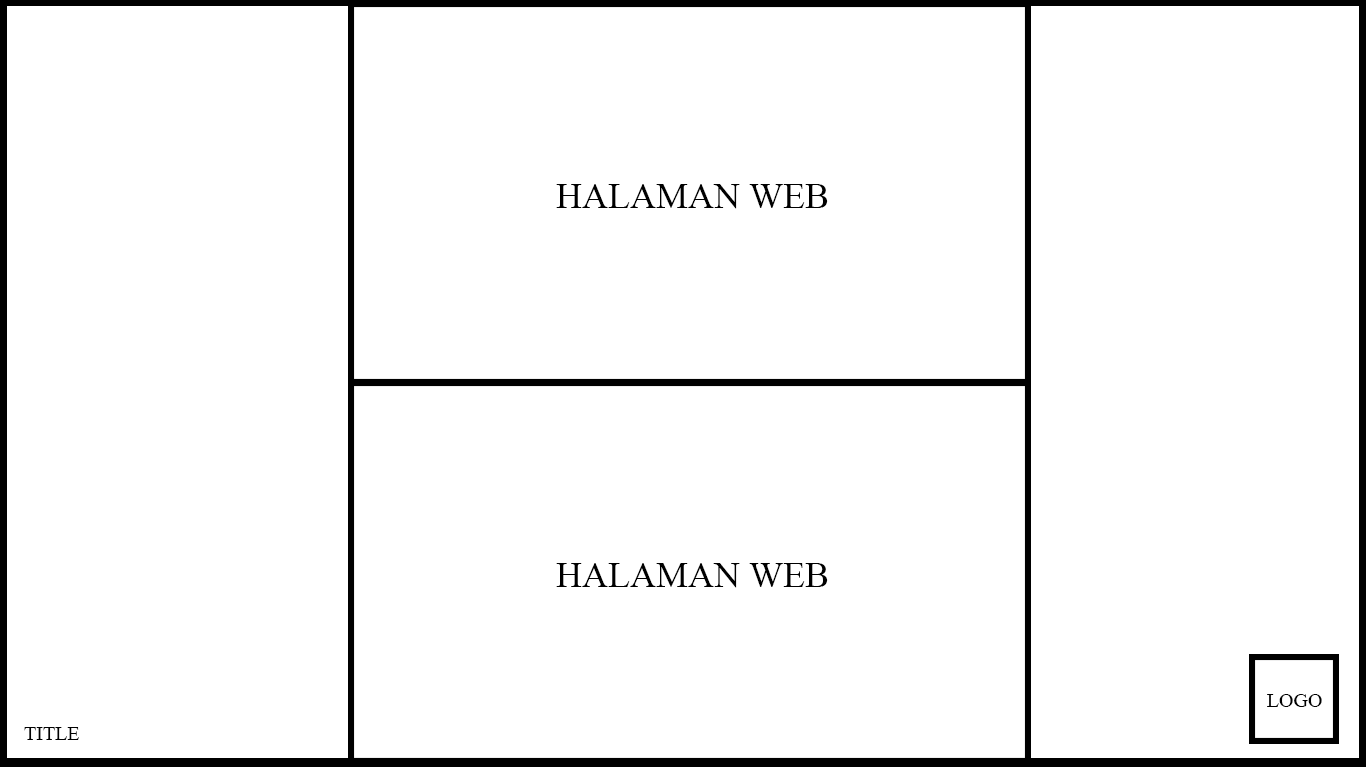
\includegraphics[scale=0.3]{Gambar/output_2.png}
	\caption{Rancangan \textit{output} jika terdapat dua halaman \textit{web}.}
	\label{fig:output2}
\end{figure}

\begin{figure}[H]
	\centering
		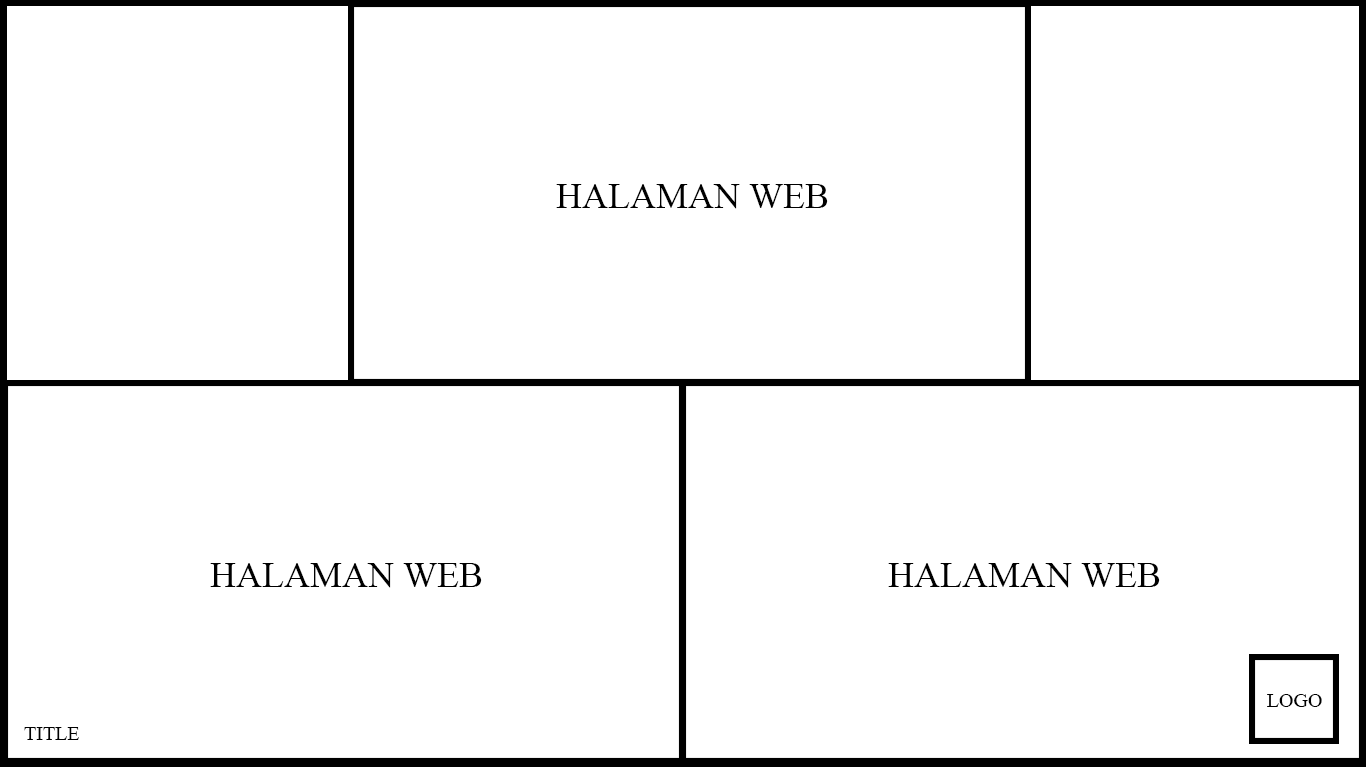
\includegraphics[scale=0.3]{Gambar/output_3.png}
	\caption{Rancangan \textit{output} jika terdapat tiga halaman \textit{web}.}
	\label{fig:output3}
\end{figure}

\begin{figure}[H]
	\centering
		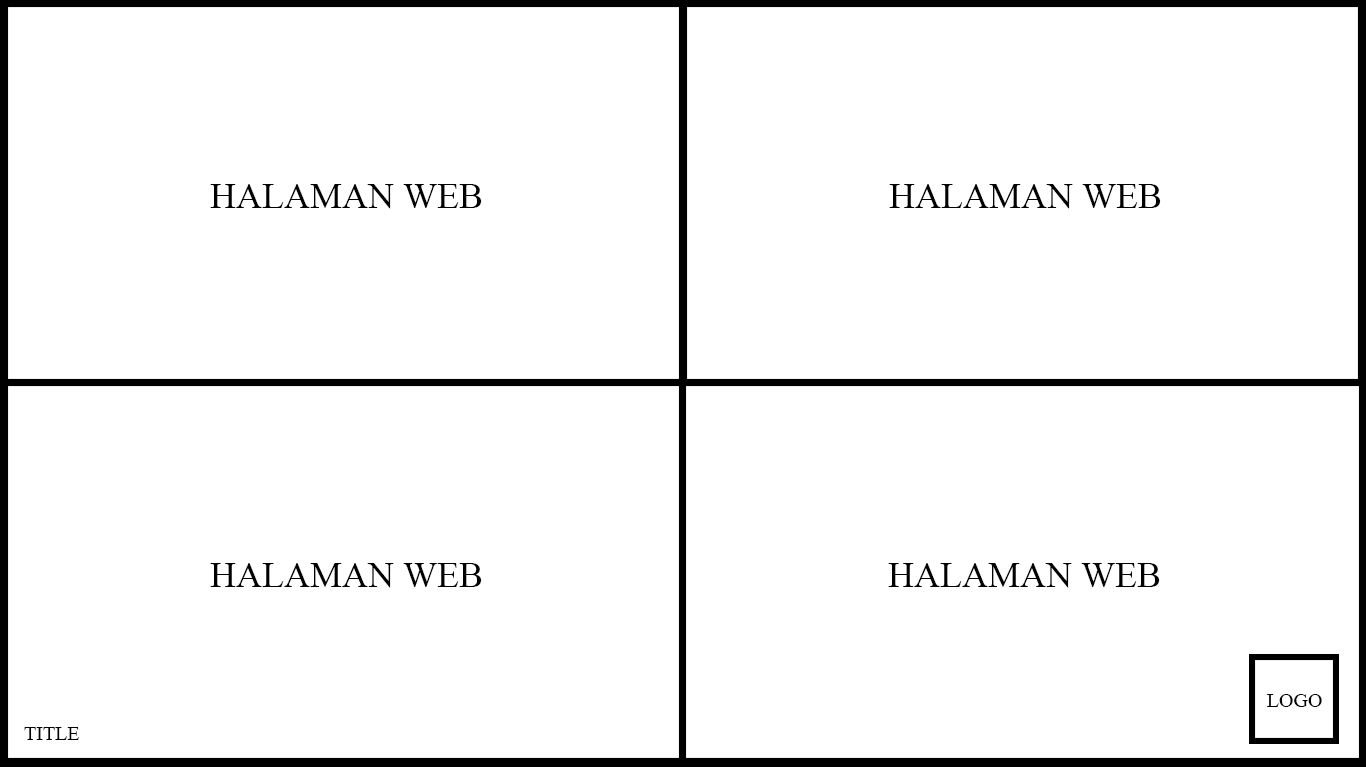
\includegraphics[scale=0.3]{Gambar/output_4.png}
	\caption{Rancangan \textit{output} jika terdapat empat halaman \textit{web}.}
	\label{fig:output4}
\end{figure}
